\section{eo\-VRP Class Reference}
\label{classeo_v_r_p}\index{eoVRP@{eoVRP}}
Defines the getoype used to solve the VRP-TW problem.  


{\tt \#include $<$eo\-VRP.h$>$}

Inheritance diagram for eo\-VRP::\begin{figure}[H]
\begin{center}
\leavevmode
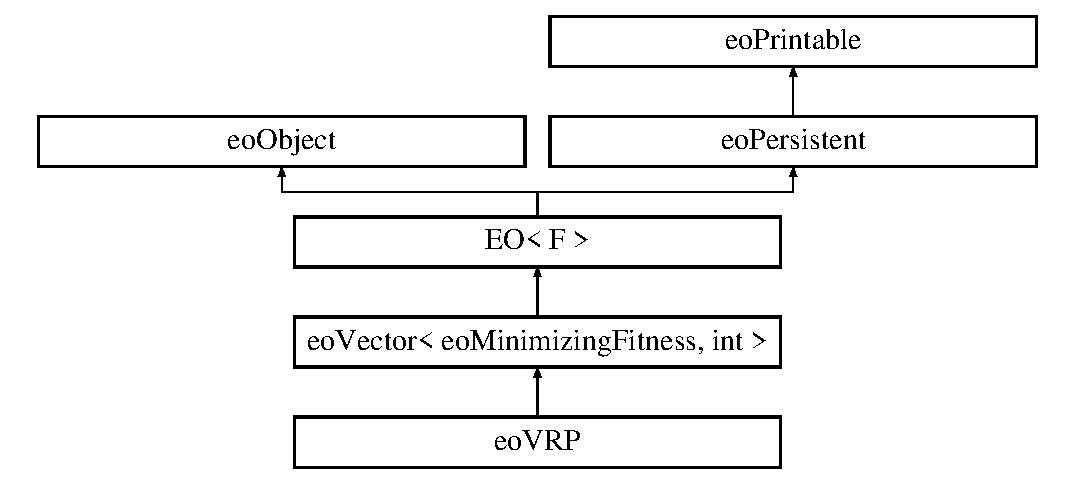
\includegraphics[height=5cm]{classeo_v_r_p}
\end{center}
\end{figure}
\subsection*{Public Member Functions}
\begin{CompactItemize}
\item 
\bf{eo\-VRP} ()\label{classeo_v_r_p_20e79a2ad5721ce7f2fe4a88f00692de}

\begin{CompactList}\small\item\em Default constructor: initializes variables to safe values. \item\end{CompactList}\item 
\bf{eo\-VRP} (const \bf{eo\-VRP} \&\_\-orig)
\begin{CompactList}\small\item\em Copy contructor: creates a new individual from a given one. \item\end{CompactList}\item 
virtual \bf{$\sim$eo\-VRP} ()\label{classeo_v_r_p_dedbd3437656d5dacafab6652219c8e2}

\begin{CompactList}\small\item\em Default destructor: nothing to do here. \item\end{CompactList}\item 
\bf{eo\-VRP} \& \bf{operator=} (const \bf{eo\-VRP} \&\_\-orig)
\begin{CompactList}\small\item\em Performs a copy from the invidual passed as argument. \item\end{CompactList}\item 
virtual std::string \bf{class\-Name} () const 
\begin{CompactList}\small\item\em Returns a string containing the name of the class. \item\end{CompactList}\item 
void \bf{print\-On} (std::ostream \&\_\-os) const 
\begin{CompactList}\small\item\em Prints the individual to a given stream. \item\end{CompactList}\item 
void \bf{print\-All\-On} (std::ostream \&\_\-os) const 
\begin{CompactList}\small\item\em Prints a detailed version of the individual (decoding information, unsatisfied contraints, etc. \item\end{CompactList}\item 
void \bf{read\-From} (std::istream \&\_\-is)
\begin{CompactList}\small\item\em Reads an individual from a given stream. \item\end{CompactList}\item 
const Routes \& \bf{routes} ()
\begin{CompactList}\small\item\em Returns a reference to the decoded individual. \item\end{CompactList}\item 
double \bf{length} ()
\begin{CompactList}\small\item\em Returns the total cost (length) of traveling all the routes. \item\end{CompactList}\item 
void \bf{print\-Routes} (std::ostream \&\_\-os) const 
\begin{CompactList}\small\item\em Aux. \item\end{CompactList}\item 
void \bf{print\-Route} (std::ostream \&\_\-os, unsigned \_\-p) const 
\begin{CompactList}\small\item\em Aux. \item\end{CompactList}\item 
bool \bf{clean} ()
\begin{CompactList}\small\item\em Cleans the individual (the vector of clients and also the decoding information). \item\end{CompactList}\item 
bool \bf{clean\-Routes} ()
\begin{CompactList}\small\item\em Invalidates the decoding information (usually after crossover or mutation). \item\end{CompactList}\item 
bool \bf{decoded} () const 
\begin{CompactList}\small\item\em Has this individual been decoded? \item\end{CompactList}\item 
bool \bf{encode} (Routes \&\_\-routes)
\begin{CompactList}\small\item\em Encodes an individual from a set of routes (usually used within crossover). \item\end{CompactList}\item 
double \bf{decode} ()
\begin{CompactList}\small\item\em Decodes an individual in a set of routes and calculates its cost (length) of traveling. \item\end{CompactList}\end{CompactItemize}
\subsection*{Private Attributes}
\begin{CompactItemize}
\item 
Routes \bf{m\-Routes}\label{classeo_v_r_p_ecbcda9f187d0d842c043544daa33558}

\begin{CompactList}\small\item\em A set of routes containing the decoding information of the individual. \item\end{CompactList}\item 
double \bf{m\-Length}\label{classeo_v_r_p_0e8c40e00bd835dd380d26d4a3abf544}

\begin{CompactList}\small\item\em Cached cost (length) of traveling the set of routes defined by the individual. \item\end{CompactList}\end{CompactItemize}


\subsection{Detailed Description}
Defines the getoype used to solve the VRP-TW problem. 



Definition at line 50 of file eo\-VRP.h.

\subsection{Constructor \& Destructor Documentation}
\index{eoVRP@{eo\-VRP}!eoVRP@{eoVRP}}
\index{eoVRP@{eoVRP}!eoVRP@{eo\-VRP}}
\subsubsection{\setlength{\rightskip}{0pt plus 5cm}eo\-VRP::eo\-VRP (const \bf{eo\-VRP} \& {\em \_\-orig})\hspace{0.3cm}{\tt  [inline]}}\label{classeo_v_r_p_1733318610dff5f47ac7d1272a4b4fb1}


Copy contructor: creates a new individual from a given one. 

\begin{Desc}
\item[Parameters:]
\begin{description}
\item[{\em \_\-orig}]The individual used to create the new one. \end{description}
\end{Desc}


Definition at line 68 of file eo\-VRP.h.

References operator=().

\subsection{Member Function Documentation}
\index{eoVRP@{eo\-VRP}!operator=@{operator=}}
\index{operator=@{operator=}!eoVRP@{eo\-VRP}}
\subsubsection{\setlength{\rightskip}{0pt plus 5cm}\bf{eo\-VRP}\& eo\-VRP::operator= (const \bf{eo\-VRP} \& {\em \_\-orig})\hspace{0.3cm}{\tt  [inline]}}\label{classeo_v_r_p_c0fcb2c17f849bfa61dd5d7ff072e0e4}


Performs a copy from the invidual passed as argument. 

\begin{Desc}
\item[Parameters:]
\begin{description}
\item[{\em \_\-orig}]The individual to copy from. \end{description}
\end{Desc}
\begin{Desc}
\item[Returns:]A reference to this. \end{Desc}


Definition at line 90 of file eo\-VRP.h.

References clean(), m\-Length, and m\-Routes.

Referenced by eo\-VRP().\index{eoVRP@{eo\-VRP}!className@{className}}
\index{className@{className}!eoVRP@{eo\-VRP}}
\subsubsection{\setlength{\rightskip}{0pt plus 5cm}virtual std::string eo\-VRP::class\-Name (void) const\hspace{0.3cm}{\tt  [inline, virtual]}}\label{classeo_v_r_p_8c7f524cf34787f9ec26ffcc420565c5}


Returns a string containing the name of the class. 

\begin{Desc}
\item[Returns:]The string containing the name of the class. \end{Desc}


Reimplemented from \bf{EO$<$ F $>$}.

Definition at line 117 of file eo\-VRP.h.\index{eoVRP@{eo\-VRP}!printOn@{printOn}}
\index{printOn@{printOn}!eoVRP@{eo\-VRP}}
\subsubsection{\setlength{\rightskip}{0pt plus 5cm}void eo\-VRP::print\-On (std::ostream \& {\em \_\-os}) const\hspace{0.3cm}{\tt  [inline, virtual]}}\label{classeo_v_r_p_dc4cb13768ef1a2c810d4d298b36707c}


Prints the individual to a given stream. 

\begin{Desc}
\item[Parameters:]
\begin{description}
\item[{\em \_\-os}]The stream to print to. \end{description}
\end{Desc}


Reimplemented from \bf{eo\-Vector$<$ eo\-Minimizing\-Fitness, int $>$}.

Definition at line 129 of file eo\-VRP.h.

References eo\-Vector$<$ Fit\-T, Gene\-Type $>$::print\-On().

Referenced by decode().\index{eoVRP@{eo\-VRP}!printAllOn@{printAllOn}}
\index{printAllOn@{printAllOn}!eoVRP@{eo\-VRP}}
\subsubsection{\setlength{\rightskip}{0pt plus 5cm}void eo\-VRP::print\-All\-On (std::ostream \& {\em \_\-os}) const\hspace{0.3cm}{\tt  [inline]}}\label{classeo_v_r_p_738f0aa43d8608cc68e41b1d3f8c944d}


Prints a detailed version of the individual (decoding information, unsatisfied contraints, etc. 

) to a given stream. \begin{Desc}
\item[Parameters:]
\begin{description}
\item[{\em \_\-os}]The stream to print to. \end{description}
\end{Desc}


Definition at line 146 of file eo\-VRP.h.

References decoded(), EO$<$ F $>$::fitness(), eo\-Vector$<$ Fit\-T, Gene\-Type $>$::print\-On(), and print\-Routes().\index{eoVRP@{eo\-VRP}!readFrom@{readFrom}}
\index{readFrom@{readFrom}!eoVRP@{eo\-VRP}}
\subsubsection{\setlength{\rightskip}{0pt plus 5cm}void eo\-VRP::read\-From (std::istream \& {\em \_\-is})\hspace{0.3cm}{\tt  [inline, virtual]}}\label{classeo_v_r_p_fdb87ffaf7ac95988e8896bb896183cc}


Reads an individual from a given stream. 

\begin{Desc}
\item[Parameters:]
\begin{description}
\item[{\em \_\-is}]The stream to read from. \end{description}
\end{Desc}


Reimplemented from \bf{eo\-Vector$<$ eo\-Minimizing\-Fitness, int $>$}.

Definition at line 177 of file eo\-VRP.h.

References eo\-Vector$<$ Fit\-T, Gene\-Type $>$::read\-From().\index{eoVRP@{eo\-VRP}!routes@{routes}}
\index{routes@{routes}!eoVRP@{eo\-VRP}}
\subsubsection{\setlength{\rightskip}{0pt plus 5cm}const Routes\& eo\-VRP::routes ()\hspace{0.3cm}{\tt  [inline]}}\label{classeo_v_r_p_0e000044813b4ebdd822e7e2f8540d8b}


Returns a reference to the decoded individual. 

\begin{Desc}
\item[Returns:]A reference to the decoded individual. \end{Desc}


Definition at line 190 of file eo\-VRP.h.

References m\-Routes.

Referenced by eo\-VRPGeneric\-Crossover::operator()().\index{eoVRP@{eo\-VRP}!length@{length}}
\index{length@{length}!eoVRP@{eo\-VRP}}
\subsubsection{\setlength{\rightskip}{0pt plus 5cm}double eo\-VRP::length ()\hspace{0.3cm}{\tt  [inline]}}\label{classeo_v_r_p_e4d189ca6349a875ae8d6fd9c7fe2491}


Returns the total cost (length) of traveling all the routes. 

\begin{Desc}
\item[Returns:]The total cost (length) of traveling all the routes. \end{Desc}


Definition at line 205 of file eo\-VRP.h.

References m\-Length.

Referenced by eo\-VRPEval\-Func::operator()().\index{eoVRP@{eo\-VRP}!printRoutes@{printRoutes}}
\index{printRoutes@{printRoutes}!eoVRP@{eo\-VRP}}
\subsubsection{\setlength{\rightskip}{0pt plus 5cm}void eo\-VRP::print\-Routes (std::ostream \& {\em \_\-os}) const\hspace{0.3cm}{\tt  [inline]}}\label{classeo_v_r_p_2a4c249cc6b15819c48c9210db385dc7}


Aux. 

method to print a structure of routes. \begin{Desc}
\item[Parameters:]
\begin{description}
\item[{\em \_\-os}]The stream to print to. \end{description}
\end{Desc}


Definition at line 217 of file eo\-VRP.h.

References m\-Routes, and print\-Route().

Referenced by print\-All\-On().\index{eoVRP@{eo\-VRP}!printRoute@{printRoute}}
\index{printRoute@{printRoute}!eoVRP@{eo\-VRP}}
\subsubsection{\setlength{\rightskip}{0pt plus 5cm}void eo\-VRP::print\-Route (std::ostream \& {\em \_\-os}, unsigned {\em \_\-p}) const\hspace{0.3cm}{\tt  [inline]}}\label{classeo_v_r_p_ec256ed5b3b15b6d220494015e2aba93}


Aux. 

method to print only one route. \begin{Desc}
\item[Parameters:]
\begin{description}
\item[{\em \_\-os}]The stream to print to. \item[{\em \_\-p}]The route to print. \end{description}
\end{Desc}


Definition at line 244 of file eo\-VRP.h.

References m\-Routes.

Referenced by print\-Routes().\index{eoVRP@{eo\-VRP}!clean@{clean}}
\index{clean@{clean}!eoVRP@{eo\-VRP}}
\subsubsection{\setlength{\rightskip}{0pt plus 5cm}bool eo\-VRP::clean ()\hspace{0.3cm}{\tt  [inline]}}\label{classeo_v_r_p_1c53a7a42174c7d40db92da644b25fec}


Cleans the individual (the vector of clients and also the decoding information). 

\begin{Desc}
\item[Returns:]True if the operation finishes correctly. False otherwise. \end{Desc}


Definition at line 267 of file eo\-VRP.h.

References m\-Length, and m\-Routes.

Referenced by encode(), eo\-VRPEdge\-Crossover::operator()(), and operator=().\index{eoVRP@{eo\-VRP}!cleanRoutes@{cleanRoutes}}
\index{cleanRoutes@{cleanRoutes}!eoVRP@{eo\-VRP}}
\subsubsection{\setlength{\rightskip}{0pt plus 5cm}bool eo\-VRP::clean\-Routes ()\hspace{0.3cm}{\tt  [inline]}}\label{classeo_v_r_p_66fb699c1d34cac859406ad450be406a}


Invalidates the decoding information (usually after crossover or mutation). 

\begin{Desc}
\item[Returns:]True if the operation finishes correctly. False otherwise. \end{Desc}


Definition at line 283 of file eo\-VRP.h.

References m\-Length, and m\-Routes.

Referenced by decode(), eo\-VRPOne\-Point\-Crossover::operator()(), and eo\-VRPMutation::operator()().\index{eoVRP@{eo\-VRP}!decoded@{decoded}}
\index{decoded@{decoded}!eoVRP@{eo\-VRP}}
\subsubsection{\setlength{\rightskip}{0pt plus 5cm}bool eo\-VRP::decoded () const\hspace{0.3cm}{\tt  [inline]}}\label{classeo_v_r_p_e188fadc91b4ee256e144ac86ee80a40}


Has this individual been decoded? 

\begin{Desc}
\item[Returns:]True if has decoding information. False otherwise. \end{Desc}


Definition at line 298 of file eo\-VRP.h.

References m\-Routes.

Referenced by eo\-VRPEval\-Func::operator()(), and print\-All\-On().\index{eoVRP@{eo\-VRP}!encode@{encode}}
\index{encode@{encode}!eoVRP@{eo\-VRP}}
\subsubsection{\setlength{\rightskip}{0pt plus 5cm}bool eo\-VRP::encode (Routes \& {\em \_\-routes})\hspace{0.3cm}{\tt  [inline]}}\label{classeo_v_r_p_b56c820bff344b4cd7338628a6f8f083}


Encodes an individual from a set of routes (usually used within crossover). 

\begin{Desc}
\item[Returns:]True if the operation finishes correctly. False otherwise. \end{Desc}


Definition at line 313 of file eo\-VRP.h.

References clean().

Referenced by eo\-VRPGeneric\-Crossover::operator()().\index{eoVRP@{eo\-VRP}!decode@{decode}}
\index{decode@{decode}!eoVRP@{eo\-VRP}}
\subsubsection{\setlength{\rightskip}{0pt plus 5cm}double eo\-VRP::decode ()\hspace{0.3cm}{\tt  [inline]}}\label{classeo_v_r_p_fdfd2633515baa85c3fdaf39be6dea5c}


Decodes an individual in a set of routes and calculates its cost (length) of traveling. 

\begin{Desc}
\item[Returns:]The cost (length) of traveling the set of routes. \end{Desc}


Definition at line 334 of file eo\-VRP.h.

References clean\-Routes(), eo\-VRPUtils::clients, eo\-VRPUtils::distance(), eo\-VRPUtils::get\-Time\-Window(), m\-Length, m\-Routes, and print\-On().

Referenced by eo\-VRPEval\-Func::operator()().

The documentation for this class was generated from the following file:\begin{CompactItemize}
\item 
eo\-VRP.h\end{CompactItemize}
